\normaltrue \difficilefalse \tdifficilefalse
\correctiontrue

%\UPSTIidClasse{11} % 11 sup, 12 spé
%\newcommand{\UPSTIidClasse}{12}

\exer{Train simple $\star$ \label{C2:06:27}}
\setcounter{question}{0}\UPSTIcompetence[2]{A3-05}
\UPSTIcompetence[2]{C2-06}
\index{Compétence C2-06}
\index{Train épicycloïdal}
\ifcorrection
\else
\marginnote{\textbf{Pas de corrigé pour cet exercice.}}
\fi

\ifprof
\else
Soit le train épicycloïdal suivant. 
\begin{center}
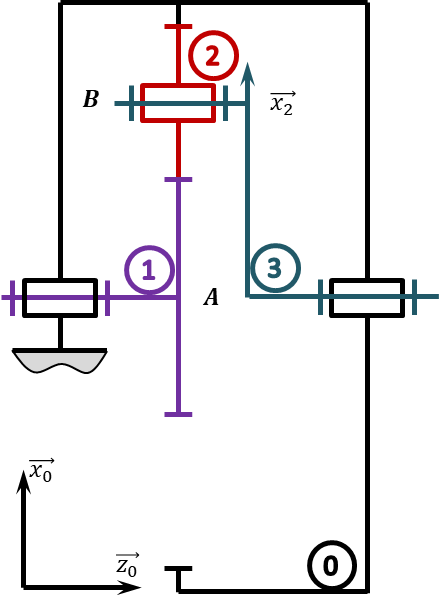
\includegraphics[width=.7\linewidth]{27_01}
\end{center}
\fi


\question{Tracer le graphe des liaisons.}
\ifprof
\else
\fi

\question{Déterminer $\dfrac{\omega_{3/0}}{\omega_{1/0}}$ en fonction du nombre de dents des roues dentées.}
\ifprof ~\\
 En bloquant le porte satellite, on a : $\dfrac{\omega_{03}}{\omega_{13}}=-\dfrac{Z_1}{Z_0}$. On a donc, 
$\dfrac{\omega_{03}}{\omega_{10}+\omega_{03}}=-\dfrac{Z_1}{Z_0}$

$\Leftrightarrow \dfrac{\omega_{30}}{\omega_{30}-\omega_{10}}=-\dfrac{Z_1}{Z_0}$
$\Leftrightarrow \omega_{30}=-\dfrac{Z_1}{Z_0} \omega_{30}+\dfrac{Z_1}{Z_0}\omega_{10} $
$\Leftrightarrow \omega_{30}\left( 1+\dfrac{Z_1}{Z_0} \right)=\dfrac{Z_1}{Z_0}\omega_{10} $
$\Leftrightarrow \omega_{30}=\dfrac{Z_1}{Z_0+Z_1}\omega_{10} $.
\else
\fi


\ifprof
\else
\begin{flushright}
\footnotesize{Corrigé  voir \ref{C2:06:27}.}
\end{flushright}%
\fi